\documentclass{article}

\usepackage{
	amsmath,
	amssymb,
	amsthm,
	bookmark,
	graphicx,
	thmtools
}
\DeclareMathOperator{\Aut}{Aut}
\DeclareMathOperator{\cdf}{cdf}
\DeclareMathOperator{\disc}{D}
\DeclareMathOperator{\GL}{GL}
\DeclareMathOperator{\tr}{tr}
\newcommand{\bF}{\mathbf{F}}
\newcommand{\bN}{\mathbf{N}}
\newcommand{\bQ}{\mathbf{Q}}
\newcommand{\bR}{\mathbf{R}}
\newcommand{\bx}{{\boldsymbol x}}
\newcommand{\by}{{\boldsymbol y}}
\newcommand{\bZ}{\mathbf{Z}}
\newcommand{\dd}{\mathrm{d}}
\newcommand{\even}{\mathrm{even}}
\newcommand{\fr}{\mathrm{fr}}
\newcommand{\Leb}{\mathrm{Leb}}
\newcommand{\odd}{\mathrm{odd}}
\newcommand{\ST}{\mathrm{ST}}

\newtheorem{corollary}[subsection]{Corollary}
\newtheorem{conjecture}[subsection]{Conjecture}
\newtheorem{lemma}[subsection]{Lemma}
\newtheorem{theorem}[subsection]{Theorem}

\title{A counterexample relating exponential sums and discrepancy}
\author{Daniel Miller}

\begin{document}
\maketitle





For a prime $p$, let 
\begin{align*}
	T_p &= \left\{ \frac{a}{2\sqrt p} : a\in \bZ, |a|\leqslant 2\sqrt p\right\} \\
	\Theta_p &= \cos^{-1}\left(T_p \right) .
\end{align*}
Since applying continuous increasing functions preserves discrepancy, we have:
\begin{align*}
	\disc(T_p,\Leb) &\ll p^{-1/2} \\
	\disc\left(\Theta_p, \frac 1 2 \sin(t)\, \dd t\right) &\ll p^{-1/2} .
\end{align*}
We claim that starting with $\theta_2\in \Theta_2$, we can choose 
$\theta_p$ such that we preserve the inequalities:
\begin{align*}
	\frac{1}{4\log x} \leqslant \disc(\{\theta_p\}_{p\leqslant x}) \leqslant \frac{4}{\log x} \\
	\left| \sum_{p\leqslant x} U_1(\theta_p)\right| \leqslant 2 \sqrt{x}
\end{align*}
Recall that 
\[
	U_1(\theta) = \frac{\sin(2\theta)}{\sin\theta} .
\]
We can run this for all $p\leqslant {10}^{5}$. Recall that 
$\pi(10^5) \approx 10000$. 

Here is what we get:
\begin{figure}[ht]
\caption{Plot of $\sum_{p\leqslant x} U_1(\theta_p)$}
\centering
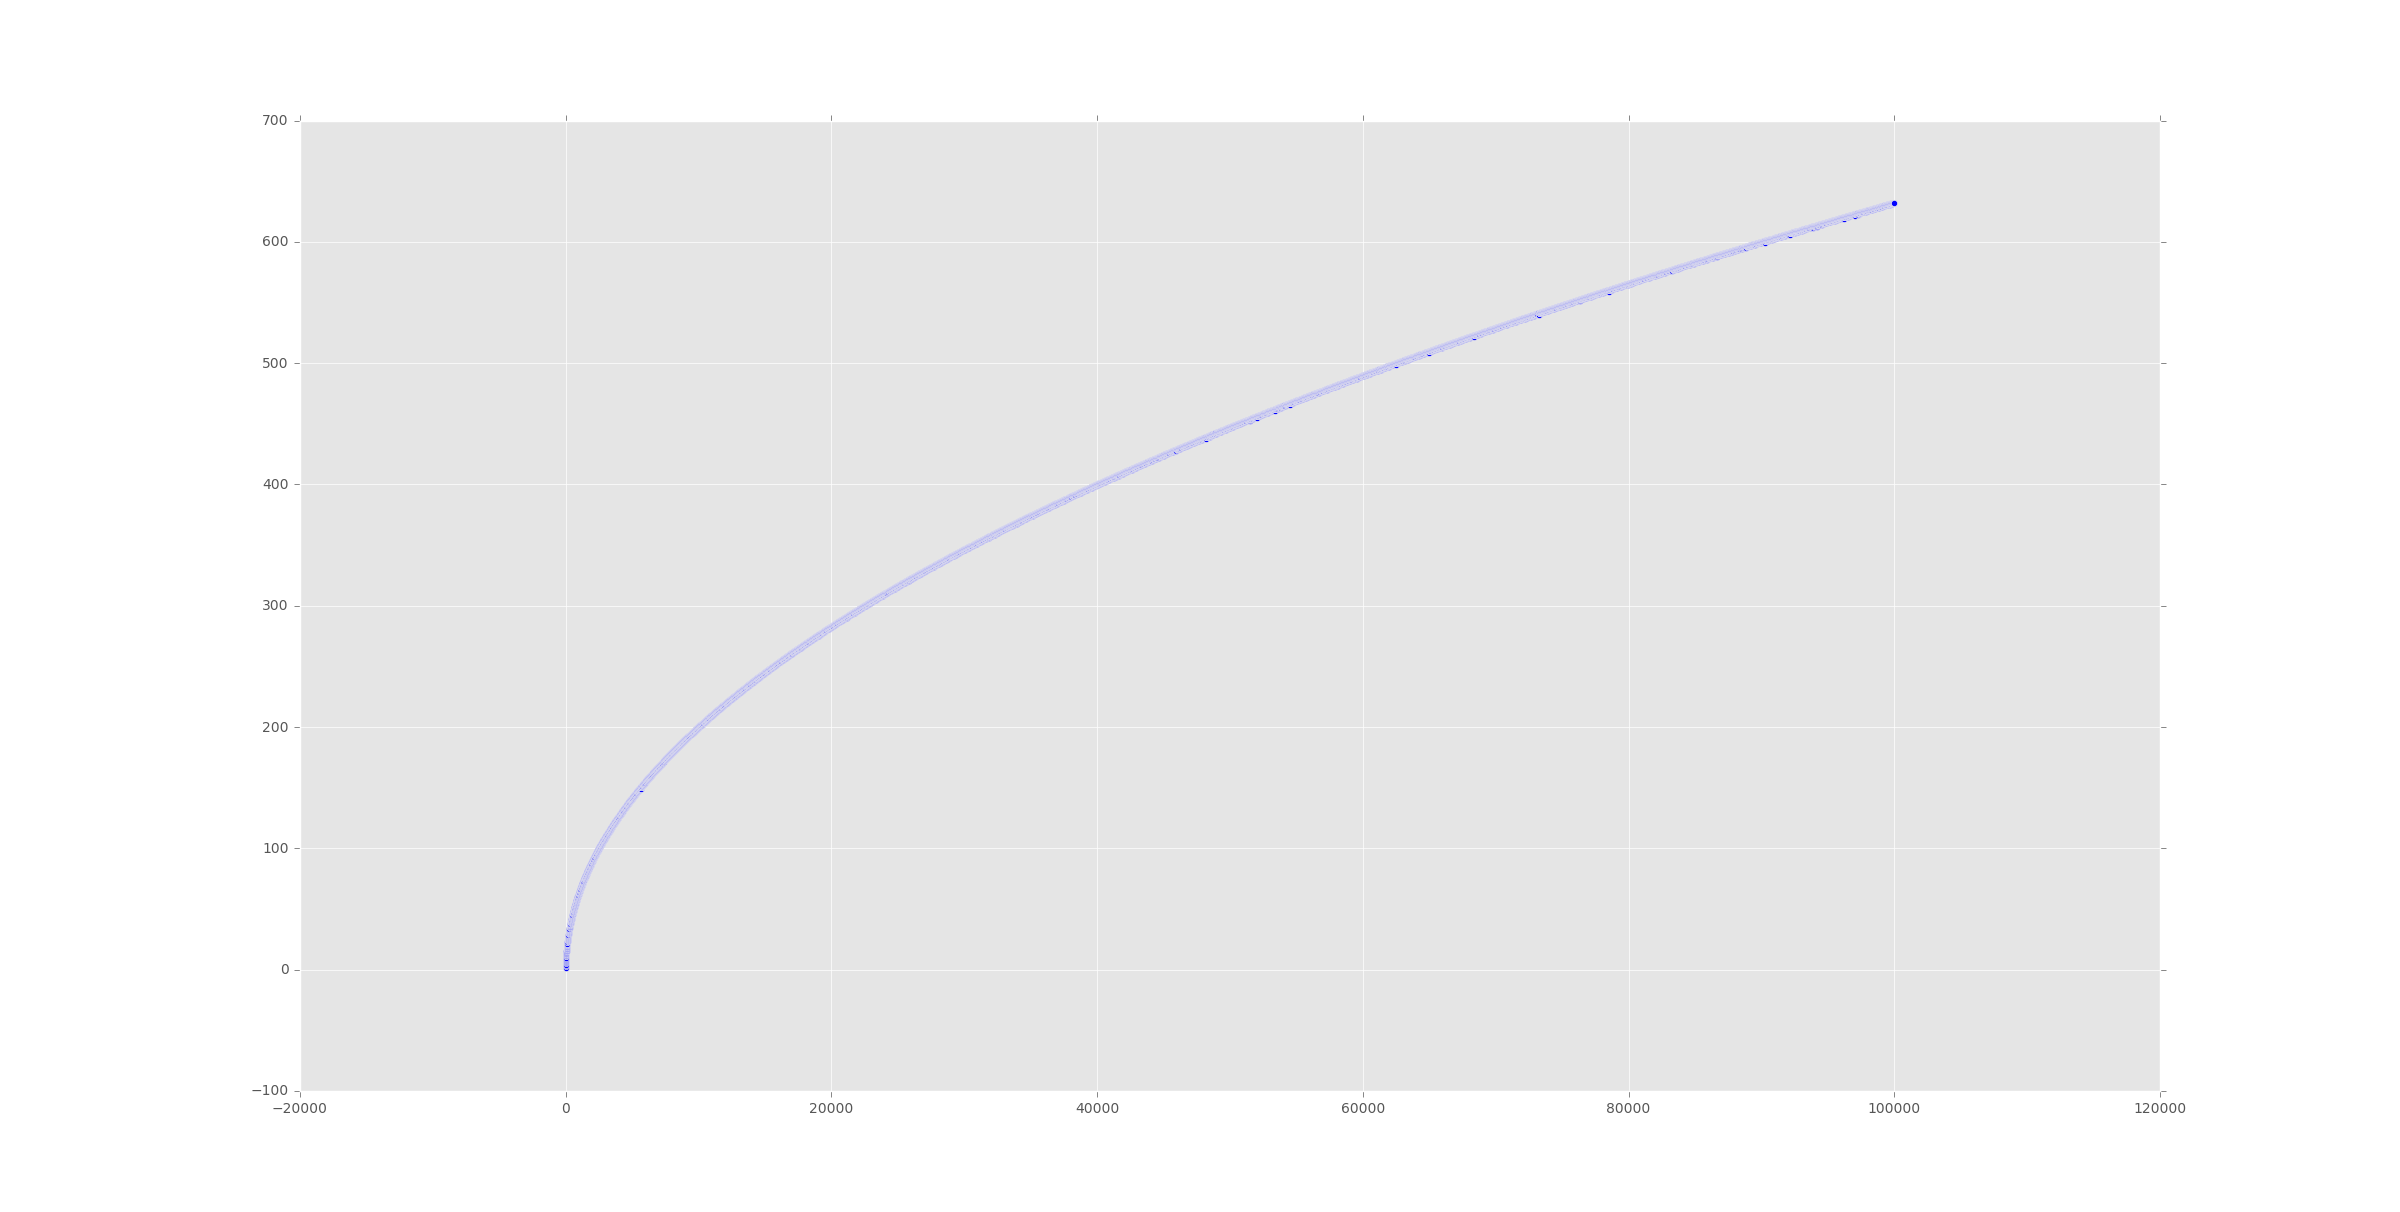
\includegraphics[width=0.8\textwidth]{sums_abs}
\end{figure}

\begin{figure}[ht]
\caption{Plot of $\disc(\{\theta_p\}_{p\leqslant x})$}
\centering
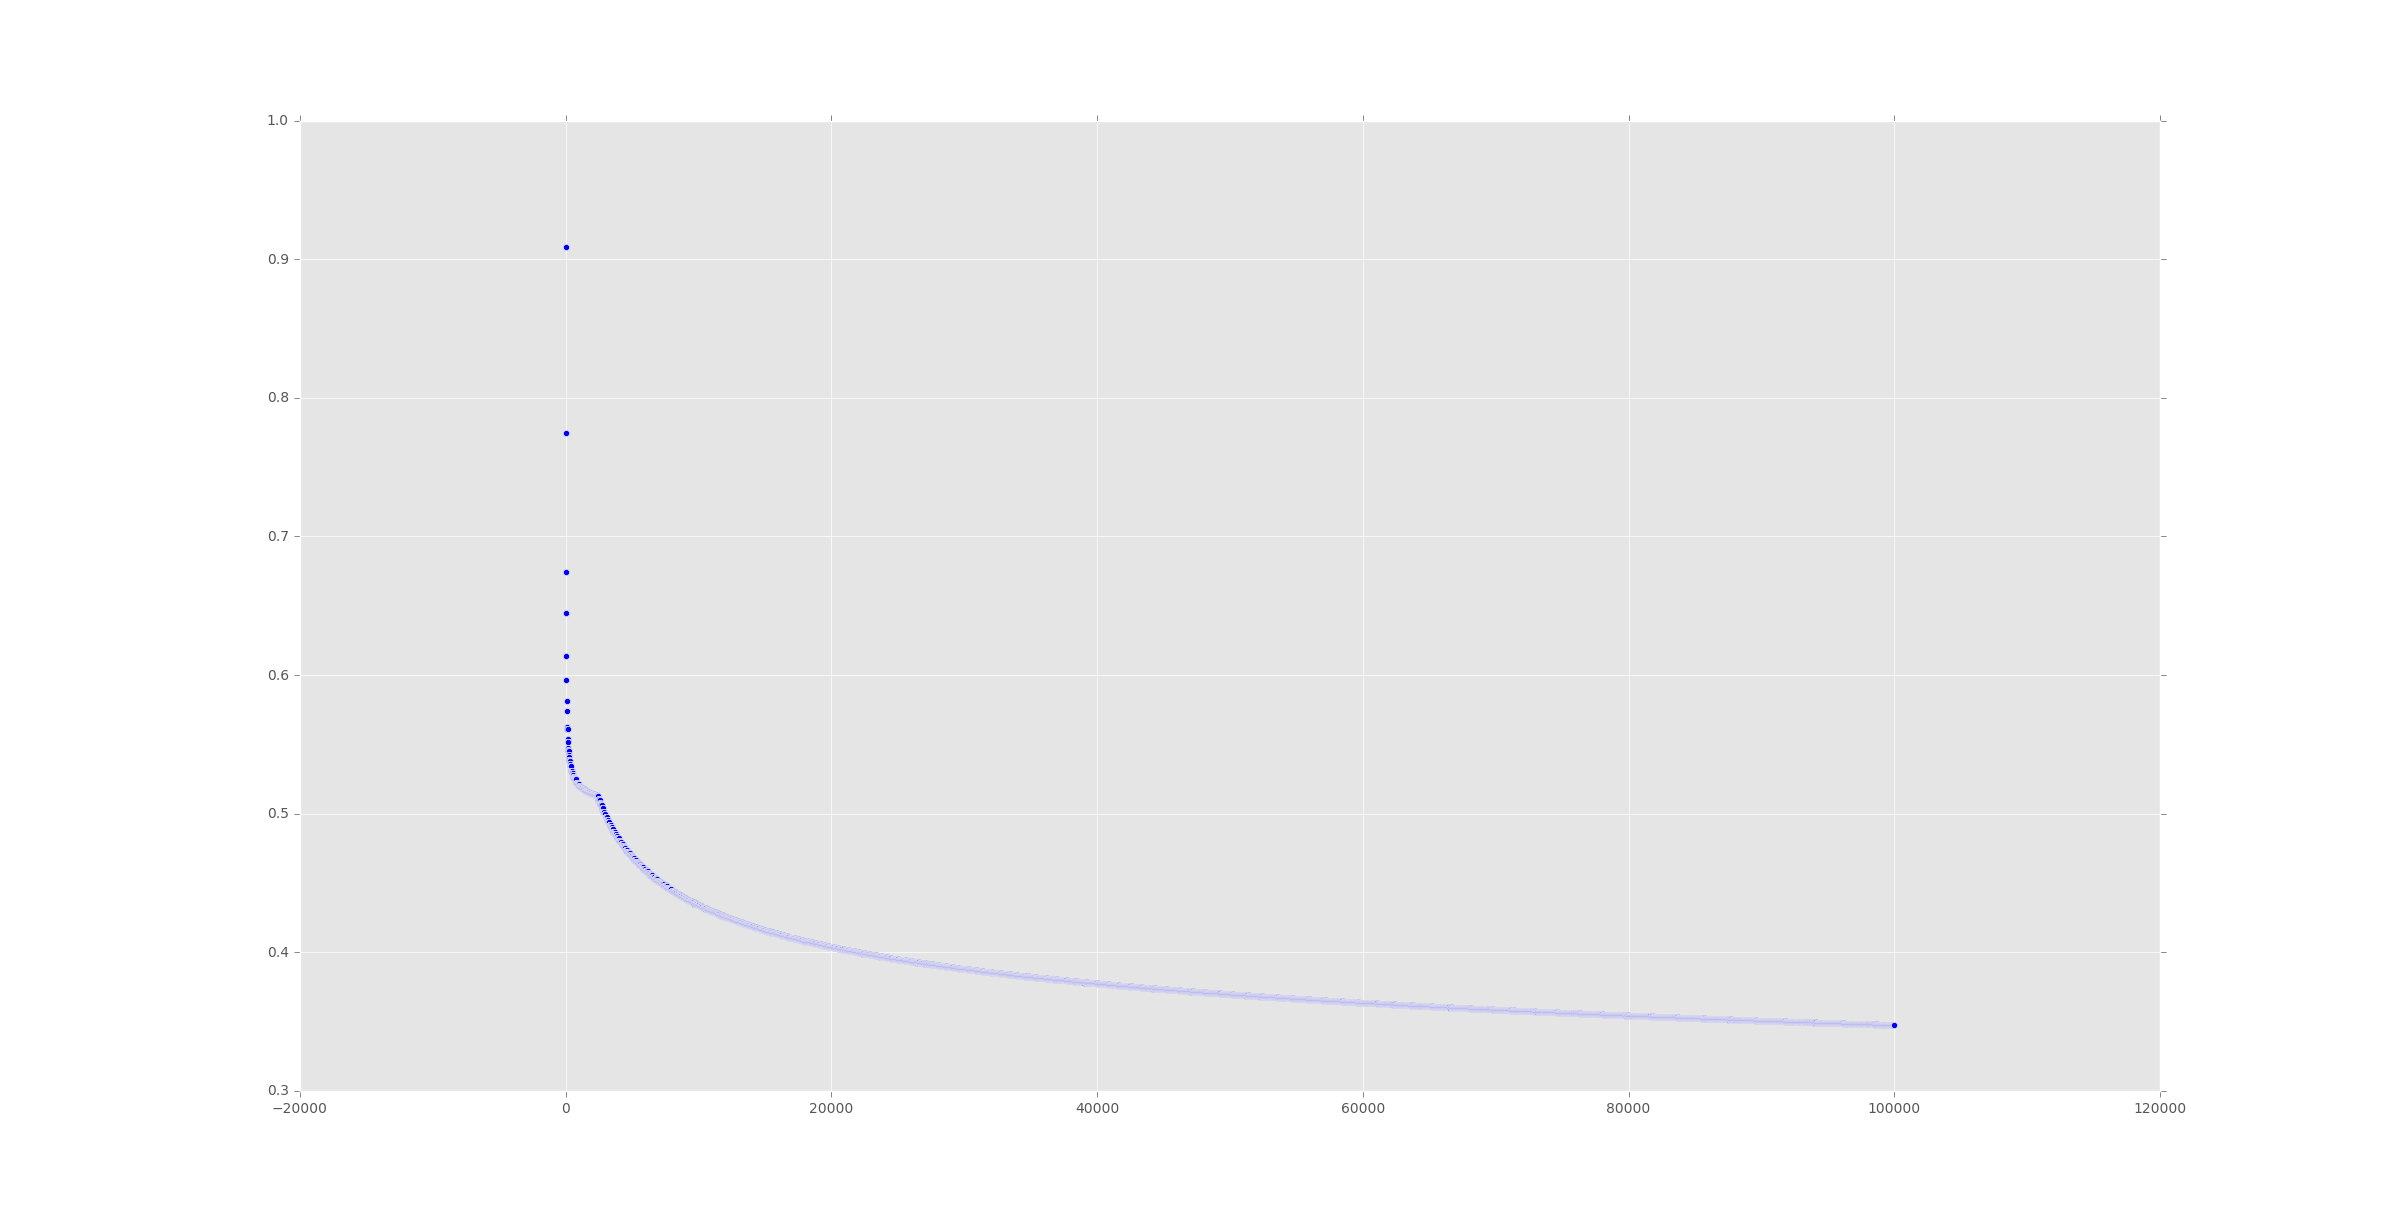
\includegraphics[width=0.8\textwidth]{ks_data}
\end{figure}

\begin{conjecture}
There exists a sequence of $\theta_p\in \Theta_p$ such that the following 
identities always hold:
\begin{align*}
	\frac{1}{4\log x} \leqslant \disc(\{\theta_p\}_{p\leqslant x}) \leqslant \frac{4}{\log x} \\
	\left| \sum_{p\leqslant x} U_1(\theta_p)\right| \leqslant 2 \sqrt{x} .
\end{align*}
\end{conjecture}

Next, choose $\bar\rho_l \colon G_\bQ \twoheadrightarrow \GL_2(\bF_l)$ to 
which we can apply Ramakrishna et.~al.'s machinery. Define 
\[
	\Theta_p(\bar\rho_l) = \left\{\cos^{-1}\left(\frac{a}{2\sqrt p}\right) : a\in \bZ, |a|\leqslant 2\sqrt p, a \equiv \tr \bar\rho_l(\fr_p)\pmod l\right\} .
\]
\begin{conjecture}
There exists a sequence of $\theta_p\in \Theta_p(\bar\rho_l)$ such that 
\begin{align*}
	\disc(\{\theta_p\}_{p\leqslant x}) =\Omega\left( \frac{1}{\log x} \right)\\
	\left| \sum_{p\leqslant x} U_1(\theta_p)\right| \ll \sqrt{x} .
\end{align*}
\end{conjecture}

\begin{corollary}
There exists an (infinitely ramified) Galois representation 
$\rho_l\colon G_\bQ \to \GL_2(\bZ_l)$ such that if we set 
$a_p = \tr\rho_l(\fr_p)$, then 
\begin{enumerate}
\item
$a_p\in \bZ$
\item
$|a_p| \leqslant 2\sqrt p$ .
\item
The $\theta_p = \cos^{-1}\left(\frac{a_p}{2\sqrt p}\right)$ satisfy 
\begin{align*}
	\disc(\{\theta_p\}_{p\leqslant x}) =\Omega\left( \frac{1}{\log x} \right)\\
	\left| \sum_{p\leqslant x} U_1(\theta_p)\right| \ll \sqrt{x} .
\end{align*}
and hence $L(\rho_l,s)$ satisfies the Riemann Hypothesis. 
\end{enumerate}
\end{corollary}





\section{Towards a proof}

Let $\bar\rho_l\colon G_\bQ \to \GL_2(\bF_l)$ be a Galois representation. For 
each prime $p$, define 
\[
	\Theta_p(l) = \left\{\cos^{-1}\left(\frac{a}{2\sqrt p}\right) : a\in \bZ, |a|\leqslant 2\sqrt p, a \equiv \tr \bar\rho_l(\fr_p)\pmod l\right\} .
\]
It is easy to check that 
\[
	\disc\left(\Theta_p(l),\frac 1 2 \sin(t)\, \dd t\right) \ll l p^{-1/2} .
\]
We are looking for a way to choose $\theta_p\in \Theta_p(l)$ such that 
\begin{enumerate}
\item
$\disc(\{\theta_p\}_{p\leqslant x})$ decays like $1/\log x$

\item
$\left| \sum_{p\leqslant x} U_1(\theta_p)\right|$ grows like 
$\sqrt x$. 
\end{enumerate}
To do this, suppose we have chosen $\{\theta_q\}_{q < p}$. In choosing 
$\theta_p$, we want to simultaneously move the discrepancy towards 
$1/\log p$, while making sure that the $U_1$-sum doesn't get too big. 

(Fact: if $\{x_1,\dots,x_N\}$ and $\{y_1,\dots,y_N\}$ are two sequences, 
then 
\[
	|\disc(\{x_1,\dots,x_N\}) - \disc(\{y_1,\dots,y_N\})| \leqslant 2\|x-y\|_\infty .
\]
)

It's actually quite simple. Note that:
\[
	U_1(\theta) = \frac{\sin(2\theta)}{\sin\theta} = -U_1(\pi-\theta) .
\]
The basic idea is: set $\theta_3 \approx \pi-\theta_2$, 
$\theta_7 \approx \pi-\theta_5$, etc.~and we can choose $\theta_2$, 
$\theta_5$ etc.~arbitrarily, meaning good discrepancy, while the sum should 
approximately cancel out. First, since $U_1$ has bounded derivative, we know 
that 
\[
	|U_1(\theta) - U_1(\varphi)| \ll |\theta-\varphi|
\]
So, if $p_1<p_2$ are sequential primes, we have 
\[
	|\theta_{p_2} - (\pi-\theta_{p_1})| \ll p_1^{-1/2} ,
\]
so 
\begin{align*}
	|U_1(\theta_{p_1}) + U_1(\theta_{p_2})| 
		&\leqslant |U_1(\theta_{p_1}) - U_1(\pi - \theta_{p_1})| + |U_1(\pi-\theta_{p_1}) - U_1(\theta_{p_2})| \\
		&\ll |\theta_{p_2} - (\pi-\theta_{p_1})| \\
		&\ll p_1^{-1/2} .
\end{align*}
So, 
\[
	\left| \sum_{p\leqslant x} U_1(\theta_p) \right| \ll \sum_{p\leqslant x} p^{-1/2} \ll \int_1^x t^{-1/2} \, \dd t \ll \sqrt x .
\]
(Same argument works for all $U_\odd$ because they all satisfy 
$U_\odd(\pi-\theta) = -U_\odd(\theta)$. In contrast, 
$U_\even(\pi-\theta) = U_\even(\theta)$.)





\section{A legit proof!}

\begin{theorem}
Fix a prime $l$. Suppose we have chosen, for all primes $p$, some arbitrary 
residue class $\bar a_p\in \bF_l$, and set 
\[
	\Theta_p(l) = \left\{\cos^{-1}\left(\frac{a}{2\sqrt p}\right) : a\in \bZ, |a|\leqslant 2\sqrt p, a \equiv \bar a_p\pmod l\right\} .
\]
Then there exists a choice of $\theta_p\in \Theta_p(l)$ such that 
\begin{enumerate}
\item
The sequence $\{\theta_p\}$ is equidistributed with respect to the Sato--Tate 
measure $\frac{2}{\pi}\sin^2\theta\, \dd \theta$. 

\item
The discrepancy $\disc(\{\theta_p\}_{p\leqslant x}, \ST) \gg \frac{1}{\log x}$. 

\item
$\left| \sum_{p\leqslant x} U_\mathrm{odd}(\theta_p)\right| \ll \sqrt x$. 
\end{enumerate}
\end{theorem}
\begin{proof}
Enumerate the primes $p_1 < p_2 < \cdots$. We will choose 
$\theta_{p_\odd}\in [0,\pi/2)$ so that the discrepancy of the sequence 
$\{\theta_{p_\odd}\}$ behaves as required in that interval. We'll then set 
$\theta_{p_{2i}}\approx \pi - \theta_{p_{2i-1}}$. 

Everything comes down to: if $p < q$ are sequential primes and we 
have already chosen $\theta_p$, we need to be able to choose $\theta_q$ so that 
$|U_1(\theta_p)+U_1(\theta_q)| \ll p^{-1/2}$. Since 
$\frac{\dd U_1}{\dd \theta} = -2\sin(\theta)$, we have (roughly)
\[
	|U_1(\theta)-U_1(\varphi)| \ll \max(\theta,\varphi) \cdot |\theta-\varphi| 
\]
for $\theta,\varphi\in [0,\pi/2)$. 

Start with $t_p = \frac{a_p}{2\sqrt p}$ and $t_q = \frac{a_q}{2\sqrt q}$. We 
can guarantee that $|t_p - (\pi-t_q)| \ll p^{-1/2}$. 

Fact: 
\[
	| \cos^{-1}(1-x) - \cos^{-1}(1-(x+\sqrt x))| \ll x^{1/5} .
\]
So roughly, 
\[
	|\theta_p - \theta_q| \ll p^{-1/5} ,
\]

After taking $\cos^{-1}$, 
all we can guarantee is that 
\[
	|\theta_p - \theta_q| \ll 
\]


--- --- --- --- --- --- --- --- --- --- --- --- 

Let's think systematically. We're picking $t_1$ and $t_2$ close to 
$1$, which is where $(\cos^{-1})'$ blows up. But there shouldn't be very many 
of them close to $1$. Aka, 
\begin{align*}
	\left|\frac{\#\{p \leqslant x : \theta_p \in [0,t)\}}{\pi(x)} - \int_0^t \dd\ST\right| 
		&\ll \frac{1}{\log x} \\ 
	\frac{\#\{p \leqslant x : \theta_p \in [0,t)\}}{\pi(x)} 
		&\ll t^2 + 	\frac{1}{\log x} .
\end{align*}

We want to know, given $x$, how small the smallest $\theta_p, p\leqslant x$ is. 
Roughly, for what $t$ is 
\[
	\# \{p \leqslant x: \theta_p\in [0,t)\} < 1? 
\]
We already know that 
\[
	\# \{p \leqslant x : \theta_p\in [0,t)\} \ll \frac{x}{\log x} \left( t^2 + \frac{1}{\log x}\right) .
\]
This is frustrating, because it means, essentially, that our convergence to 
the Sato--Tate measure is so slow (by design) that we can't \emph{ever} 
guarantee that no $\theta_p$ lies in some small interval. But there's 
something easier. For each $p\leqslant x$, we start by choosing 
$a_p\in \bZ$. How close can $a_p$ be to $2\sqrt p$? Numerical experiments 
\textbf{(prove this!)} show that for $t_p = \frac{a_p}{2\sqrt p}$, we have 
\[
	|1-t_p| \gg p^{-1/2} .
\]
This is key! That means $\theta_p$ won't be too small. In particular, we 
can control how close $\theta_p$ and $\theta_q$ will be. 

We already have chosen $\theta_p$. We want to choose $a_q$ so that 
$\cos^{-1}(\frac{a_q}{2\sqrt q}) \approx \pi-\theta_p$, i.e.
\[
	\frac{a_q}{2\sqrt q} \approx \sin(\theta_p) .
\]
We can ensure 
\[
	\left| \frac{a_q}{2\sqrt q} - \cos(\pi - \theta_p)\right| \ll p^{-1/2} .
\]
Moreover, we know that $|\pm 1 - \frac{a_q}{2\sqrt q}| \gg q^{-1/2}$, and 
likewise for $a_p$. Thus, 
\[
	|\theta_p - \theta_q| = \left|\cos^{-1}\left(\frac{a_p}{2\sqrt p}\right) - \pi +  \cos^{-1}\left(\frac{a_q}{2\sqrt q}\right)\right| \ll p^{-1/2} \cdot ?
\]

Good news: numerical experiments show that we can get very good approximation 
to $U_1(\theta_q) \approx - U_1(\theta_p)$ for $p<q$ successive primes. This 
is fantastic!

Numerical experiments suggest that we can enforce 
\[
	|U_1(\theta_p)+U_1(\theta_q)| \ll \frac{\log p}{p} .
\]
\end{proof}

Let $(X,\mu)$ be a topological measure space. Suppose $g$ is a non-trivial 
automorphism of $X$, such that $g_\ast \mu = \mu$. Suppose $g^2=1$. If we 
want to minimize 
\[
	\left| \sum_{p\leqslant x} f(x_p)\right| ,
\]
while letting the discrepancy of $\{x_p\}$ vary arbitrarily. Suppose we can 
find a ``good'' subset $U\subset X$ such that $X = U \sqcup g U$. Choose 
$x_{p_\odd}\in U$ to control the discrepancy, and then choose 
$x_{p_\even} \approx g(x_{p_\odd})$. For any $f\in C^\infty(X)$ such that 
$g^\ast f = - f$. Then 
\[
	\sum_{p\leqslant x} f(x_p) = \sum (f(x_{p_\even}) + f(x_{p_\odd})) \approx \sum 0 .
\]

We know that near $\theta=0$, 
\[
	U_n(\theta) = n + C_n \theta^2 + O(\theta^3) .
\]
(I think this will hold for any $f$ with $\int f=0$ and
$f(\pi-\theta)=f(\theta)$.)





\section{Precise method}

Let $\{p_1,p_2,\dots,\}$ be an enumeration of the rational primes. Given 
$x\in \bR$, write $\sum_{p_\odd \leqslant x} a_p$ for the sum of all $a_p$ 
for $p_i\leqslant x$ with $i$ odd, and similarly for 
$\sum_{p_\even\leqslant x}$. Suppose we have chosen 
$\theta_{p_\odd}\in [0,\pi/2)$ so that 
$\disc(\{\theta_{p_\odd}\}_{p_\odd \leqslant x})$ decays as desired. Suppose 
we choose $\theta_{p_\even} \approx \pi - \theta_{p_\odd}$. That is, for 
$p < q$ successive primes with $p=p_i$, $i$ odd, we'll choose 
$\theta_q \approx \pi - \theta_p$. 

We know that $\theta_p = \cos^{-1}\left(\frac{a_p}{2\sqrt p}\right)$ for 
some $a_p\in \bZ$ with $|a_p| \leqslant 2\sqrt p$. We want to choose 
$\theta_q\approx \pi-\theta_p$, i.e.~
\begin{align*}
	\cos^{-1}\left(\frac{a_q}{2\sqrt q}\right) 
		&\approx \pi - \cos^{-1}\left(\frac{a_p}{2\sqrt p}\right) \\
	\frac{a_q}{2\sqrt q} 
		&\approx -\frac{a_p}{2\sqrt p} .
\end{align*}
since $\cos(\pi - \cos^{-1}(x)) = - x$. We can guarantee that 
\[
	\left|\frac{a_q}{2\sqrt q} + \frac{a_p}{2\sqrt p}\right| \leqslant \frac{1}{\sqrt q} .
\]

Claim: if $x,y$ are ``further than $\epsilon$'' from $\pm 1$ and 
$|x-y|<\epsilon$, then 
$|\cos^{-1}(x) - \cos^{-1}(y)| \leqslant \sqrt \epsilon$. 
(Have checked with Wolfram Alpha, prove later.)

In conclusion, for each successive primes $p=p_\odd < q=p_\even$, if there 
is $\theta_p\in \Theta_p(l)$ chosen already, we can also choose 
$\theta_q\in \Theta_q(l)$ so that 
\[
	|\theta_q - (\pi - \theta_p)| \ll l p^{-1/4} .
\]
This is all that is needed, since we're looking at $f$ that is of the form 
\[
	f(\theta) = f(0) + C \theta^2 + O(\theta^3)
\]
for $\theta$ close to zero. (In fact, this is true for \emph{all} smooth, 
Weyl-invariant $f$, whether or not they satisfy $f(\theta) = -f(\pi-\theta)$.)
The squaring ``pushes the difference'' back to 
$p^{-1/2}$. That is, for $\theta,\varphi$ close to zero, but at least 
$\epsilon$ away from zero, we have 
\[
	|f(\theta) - f(\varphi)| \ll |\theta-\varphi|^2 .
\]
Now the question is, if $\theta_q \approx \pi - \theta_p$, how close is the 
discrepancy of $\{\theta_{p_\odd}\}$ and $\{\theta_{p_\even}\}$?

Better, how close are 
\[
	\# \{p_\odd \leqslant x : \theta_{p_\odd} \leqslant t\} \qquad \textnormal{and}\qquad \# \{p_\odd \leqslant x : \theta_{p_\odd} \leqslant t\} ?
\]
We know that $|\theta_p - \theta_q| \ll p^{-1/4}$. Actually, all we need is 
that if $\disc(\{\theta_{p_\odd}\}) \to 0$, then also 
$\disc(\{\theta_{p_\even}\}) \to 0$. 

Suppose we have two sequences $\{x_n\}$ and $\{y_n\}$ such that  
$\disc(\{x_n\}_{n\leqslant N}) \sim \frac{1}{\log N}$, and also 
$|x_n - y_n| \leqslant n^{-1/4}$. For some really big $N$, choose 
$M<N$, ideally $M\approx \log N$. 

Look at 
\[
	\limsup_{N\to \infty} \disc(\{y_n\}_{M\leqslant n \leqslant N}) \leqslant M^{-1/4} .
\]
With complete generality, we have:
\[
	\left|\disc(\{x_n\}_{n\leqslant N}) - \disc(\{x_n\}_{M\leqslant n\leqslant N})\right| \ll \frac{1}{M}
\]
This is all we need.



\begin{lemma}\label{lem:compare-disc}
Let $\bx$ and $\by$ be sequences in $\bR_{\geqslant 0}$. Suppose 
$\nu = f\, \dd x$ for a continuous function $f$. Then 
\[
	|\disc^\star(\bx^N,\nu) - \disc^\star(\by^N,\nu)| \leqslant \epsilon\|f\|_\infty + \frac{\# \{n\leqslant N : |x_n - y_n| > \epsilon\}}{N} .
\]
\end{lemma}
\begin{proof}
It is actually sufficient to just prove that 
\[
	\disc^\star(\by^N,\nu) \leqslant \disc^\star(\bx^N,\nu) + \epsilon \|f\|_\infty + \frac{\# \{n\leqslant N : |x_n - y_n| > \epsilon\}}{N} .
\]
Start with an arbitrary interval $[0,t)$. Clearly 
\[
	\# \{n\leqslant N : y_n < t\} \leqslant \# \{ n\leqslant N : x_n < t + \epsilon\} + \# \{n\leqslant N : |x_n - y_n| > \epsilon\} ,
\]
and also 
\[
	\left|\frac{\#\{n\leqslant N : x_n < t+\epsilon\}}{N} - \mu[0,t+\epsilon)\right| \leqslant \disc^\star(\bx^N,\mu) .
\]
It follows that 
\[
	\frac{\#\{n\leqslant N : y_n < t\}}{N} - \mu[0,t) \leqslant \mu[t,t+\epsilon) + \disc^\star(\bx^N,\mu) + \frac{\#\{n\leqslant N : |x_n - y_n| > \epsilon\}}{N} .
\]
A similar argument with $[0,t-\epsilon)$ yields 
\[
	\frac{\#\{n\leqslant N : y_n < t\}}{N} - \mu[0,t) \geqslant -\mu[t-\epsilon,t) - \disc^\star(\bx^N,\mu) - \frac{\#\{n\leqslant N : |x_n - y_n| > \epsilon\}}{N} .
\]
Since the discrepancy is a supremum over $t$, we get 
\[
	\disc^\star(\by^N,\mu) \leqslant \disc^\star(\bx^N,\mu) + \|f\|_\infty \epsilon + \frac{\#\{n\leqslant N : |x_n - y_n| > \epsilon\}}{N}
\]
as desired. 
\end{proof}

This lemma has a powerful application. 

\begin{theorem}\label{thm:two-discrepancies}
Let $\bx$ and $\by$ be sequences in $\bR$ and $\mu = f\, \dd x$ be a measure 
induced by a continuous function $f$. Suppose that 
\begin{enumerate}
\item
$\bx$ is $\mu$-equidistributed. 
\item
$\|\bx_{>N} - \by_{>N}\|_\infty \to 0$. 
\end{enumerate}
Then $\by$ is also $\mu$-equidistributed. 
\end{theorem}
\begin{proof}
Recall that $\bx_{>N} = (x_{N+1}, x_{N+2},\dots)$, and that $\|\cdot\|_\infty$ 
is the supremum norm. Let $\varphi:\bN \to \bN$ be a function such that 
$\varphi(n) \to \infty$, but also $\varphi(n) = o(n)$. For example, we could 
have $\varphi(n) = \lfloor \log n\rfloor$. For any $N$, let 
$\epsilon = \|\bx_{>\varphi(N)} - \by_{>\varphi(N)}\|_\infty$, and apply 
\autoref{lem:compare-disc}. Trivially, we know that 
\[
	\#\{n\leqslant N : |x_n - y_n| > \epsilon\} \leqslant \varphi(N) ,
\]
so we can write 
\[
	\disc(\by^N,\mu) \leqslant \disc(\bx^N,\mu) + 2 \|\bx_{> \varphi(N)} - \by_{> \varphi(N)}\|_\infty \cdot \|f\|_\infty + \frac{\varphi(N)}{N} \to 0 .
\]
Note that we do not control the rate of decay of $\disc(\by^N,\mu)$. 
\end{proof}





\section{Summary of argument}

Fix a prime $l$, and for each prime $p$, a choice of equivalence class 
$\bar a_p \in \bF_l$. Define 
\[
	\Theta_p(l) = \left\{ \cos^{-1}\left( \frac{a}{2\sqrt p}\right) : a\in \bZ, |a|\leqslant 2\sqrt p, a\equiv \bar a_p \pmod l\right\} .
\]
Claim: there is a choice of $\theta_p\in \Theta_p(l)$ such that 
\begin{enumerate}
\item
$\disc^\star(\{\theta_p\}_{p\leqslant X})$ is not $O(X^{-\epsilon})$ for any 
$\epsilon>0$. 

\item
For any $f\in C^\infty(\bR/2\pi \bZ)^W$ with $f(\pi-\theta) = -f(\theta)$, we 
have 
\[
	\left| \sum_{p\leqslant X} f(\theta_p)\right| \ll \sqrt X .
\]
\end{enumerate}

How do we construct this sequence $\{\theta_p\}_p$? Enumerate the primes as 
$\{p_n\}_{n\geqslant 1}$. Choose the sequence 
$\{\theta_{p_{2 n-1}}\}_{n\geqslant 1}$ so that 
\begin{enumerate}
\item
$\theta_{p_{2n-1}}\in [0,2\pi)$
\item
$\disc^\star\left(\{\theta_{p_{2n-1}}\}_{n\leqslant N}, 2\cdot \ST|_{[0,\pi/2)}\right) \to 0$, but slower 
than any $N^{-\epsilon}$. \textbf{(Prove this is possible!)} 
\end{enumerate}
We've proved that we can choose $\theta_{p_{2n}}$ so that 
$|\theta_{p_{2n}} - (\pi - \theta_{p_{2n-1}})| \ll l p^{-1/4}$, which 
implies (via \autoref{thm:two-discrepancies}) that 
\[
	\disc^\star\left(\{\theta_{p_{2n}}\}_{n\leqslant N}, 2\cdot \ST|_{[\pi/2,\pi)}\right) \to 0 .
\]
\textbf{(We need to know that the discrepancy of $\pi/2-\bx$ is the same as 
that of $\bx$.)} It follows that the sequence $\{\theta_p\}$ formed by 
interleaving our ``even'' and ``odd'' indexed primes has discrepancy that 
goes to zero \textbf{(We need to prove that if $\bx$ and $\by$ are sequences 
equidistributed with respect to measures supported on $[0,\pi/2)$ and 
$[\pi/2,\pi)$, then the ``interleaved'' sequence also has equidistribution 
and discrepancy which decays no faster than the slower of the two.)}

Note that our hypothesis on $\theta_{p_{2n}}\approx \pi - \theta_{p_{2n-1}}$, 
we have, for $f$ as in the result,  
\[
	|f(\theta_{p_{2n-1}}) + f(\theta_{p_{2n}})| \ll_f l p^{-1/2} .
\]
\textbf{(Problem here: this bound only works near ``the edges.'' But also, 
the $\theta$s are better away from the edges.)}

Answer to the last problem: once we've chosen $f$, we know that it's Taylor 
expansions (hence nice bounds) converge within some neighborhood of $0$ and 
$\pi$. Outside those neighborhoods, our ``transformation function'' is smooth 
and so we can choose the $\theta_q$ to be within $O(p^{-1/2})$ of $\theta_p$. 
Also, $f$ has bounded derivatives away from those neighborhoods, so the 
$f(\theta_q)$ and $-f(\theta_p)$ are also sufficiently close. Everything works!





\end{document}
